\begin{tikzpicture}

\begin{axis}[
width=1.00\textwidth,
height=8cm,
name=statSphere,
%~ scale only axis,
ylabel=${u_{\mathrm{y}}\,\mathrm{[L\,T^{-1}]}}$,
%~ xlabel=${\ell\,\mathrm{[1]}}$,
xticklabels={,,},
%~ xmajorgrids,
xmin = 0.0,
xmax = 1.00,
ymin = -0.31,
ymax = 0.31,
y tick label style={
                /pgf/number format/.cd,
                fixed,
                fixed zerofill,
                precision=1,
                /tikz/.cd
            },
legend style ={
                at={(0.01,0.02)}, 
                anchor=south west, %north west
                font=\small
            },
cycle list name=exotic,
]
\node [anchor=center] (figA) at (rel axis cs:0.5,0.5) {
\includegraphics[width=0.355\textwidth]{\myGraphs/staticSphere/30_SphereCR.png}};

\addlegendimage{line legend,thick,black}
\addlegendentry{$\Rey = 100 $ }
\addlegendimage{line legend,thick,dashed,black}
\addlegendentry{$\Rey = 500 $ }

\addplot+ [mark=none,blue,style=solid,thick]table [x expr=\thisrow{l}/100, y={Uy}] {\myGraphs/staticSphere/POL_X_CFD_Re_100};
\label{RE100}

\addplot+ [mark=none,blue,style=thick,dashed]table [x expr=\thisrow{l}/100, y={Uy}] {\myGraphs/staticSphere/POL_X_CFD_Re_500};
\label{RE500}

\addplot+ [mark=none,red,style=solid,thick]table [x expr=\thisrow{l}*10, y={Uy}] {\myGraphs/staticSphere/POL_X_Hex_Re_100_V18-V8-DEV1OF6};
\label{R1}
\addplot+ [mark=none,red,style=solid,dashed,thick]table [x expr=\thisrow{l}*10, y={Uy}] {\myGraphs/staticSphere/POL_X_Hex_Re_500_V18-V8-DEV1OF6};

%tri
\addplot+ [mark=none,green,style=solid,thick]table [x expr=\thisrow{l}*10, y={Uy}] {\myGraphs/staticSphere/POL_X_tri_Re_100_V18-V8-DEV1OF6};
%tri
\label{R2}
%tri
\addplot+ [mark=none,green,style=solid,dashed,thick]table [x expr=\thisrow{l}*10, y={Uy}] {\myGraphs/staticSphere/POL_X_tri_Re_500_V18-V8-DEV1OF6};

%poly
\addplot+ [mark=none,brown,style=solid,thick]table [x expr=\thisrow{l}*10, y={Uy}] {\myGraphs/staticSphere/POL_X_poly_Re_100_V18-V8-DEV1OF6};
%poly
\label{R3}
%poly
\addplot+ [mark=none,brown,style=solid,dashed,thick]table [x expr=\thisrow{l}*10, y={Uy}] {\myGraphs/staticSphere/POL_X_poly_Re_500_V18-V8-DEV1OF6};

\node [draw,fill=white,anchor=north east,font=\small] at (rel axis cs: 0.99,0.98) {\shortstack[l]
{
\ref{RE100} CFD \\
\ref{R1} hexMesh \\ 
\ref{R2} triMesh \\
\ref{R3} polyMesh  
%merged\ref{R4} $\mathrm{U_{}^{mergedMesh}}$
}};

\node [draw,fill=white,anchor=south] at (rel axis cs: 0.5,0.02) {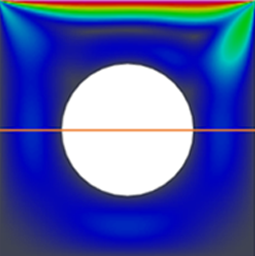
\includegraphics[width=0.22\textwidth]{\myGraphs/staticSphere/30_SubPlotA.png}};

\end{axis}

\begin{axis}[
width=1.00\textwidth,
height=8cm,
name=statImp,
at=(statSphere.below south),anchor=above north,
%~ scale only axis,
ylabel=${u_{\mathrm{y}}\,\mathrm{[L\,T^{-1}]}}$,
xlabel=${\ell\,\mathrm{[L]}}$,
%~ xticklabels={,,},
%~ xmajorgrids,
xmin = 0.0,
xmax = 1.00,
ymin = -0.31,
ymax = 0.31,
y tick label style={
                /pgf/number format/.cd,
                fixed,
                fixed zerofill,
                precision=1,
                /tikz/.cd
            },
legend style ={
                at={(0.01,0.02)}, 
                anchor=south west, %north west
                font=\small
            },
cycle list name=exotic,
]
\node [anchor=center] (figB) at (rel axis cs:0.5,0.5) {
\includegraphics[width=0.33\textwidth]{\myGraphs/staticImpeller/15_ImpellerCR.png}};

\addlegendimage{line legend,thick,black}
\addlegendentry{$\Rey = 100 $ }
\addlegendimage{line legend,thick,dashed,black}
\addlegendentry{$\Rey = 500 $ }

\addplot+ [mark=none,blue,style=solid,thick]table [x expr=\thisrow{l}/100, y={Uy}] {\myGraphs/staticImpeller/POL_X_CFD_Re_100};

\addplot+ [mark=none,blue,style=thick,dashed]table [x expr=\thisrow{l}/100, y={Uy}] {\myGraphs/staticImpeller/POL_X_CFD_Re_500};

\addplot+ [mark=none,red,style=solid,thick]table [x expr=\thisrow{l}/100, y={Uy}] {\myGraphs/staticImpeller/POL_X_Hex_Re_100_V18-V8-DEV1OF6};

\addplot+ [mark=none,red,style=solid,dashed,thick]table [x expr=\thisrow{l}/100, y={Uy}] {\myGraphs/staticImpeller/POL_X_Hex_Re_500_V18-V8-DEV1OF6};

%tri
\addplot+ [mark=none,green,style=solid,thick]table [x expr=\thisrow{l}/100, y={Uy}] {\myGraphs/staticImpeller/POL_X_tri_Re_100_V18-V8-DEV1OF6};
%tri
%tri
\addplot+ [mark=none,green,style=solid,dashed,thick]table [x expr=\thisrow{l}/100, y={Uy}] {\myGraphs/staticImpeller/POL_X_tri_Re_500_V18-V8-DEV1OF6};

%poly
\addplot+ [mark=none,brown,style=solid,thick]table [x expr=\thisrow{l}/100, y={Uy}] {\myGraphs/staticImpeller/POL_X_poly_Re_100_V18-V8-DEV1OF6};
%poly
\label{R3}
%poly
\addplot+ [mark=none,brown,style=solid,dashed,thick]table [x expr=\thisrow{l}/100, y={Uy}] {\myGraphs/staticImpeller/POL_X_poly_Re_500_V18-V8-DEV1OF6};

\node [draw,fill=white,anchor=north east,font=\small] at (rel axis cs: 0.99,0.98) {\shortstack[l]
{
\ref{RE100} CFD \\
\ref{R1} hexMesh \\ 
\ref{R2} triMesh \\
\ref{R3} polyMesh  
%merged\ref{R4} $\mathrm{U_{}^{mergedMesh}}$
}};

\node [draw,fill=white,anchor=south] at (rel axis cs: 0.5,0.02) {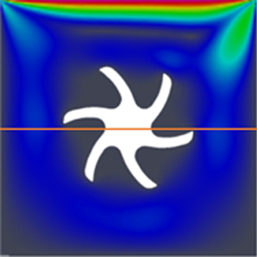
\includegraphics[width=0.22\textwidth]{\myGraphs/staticImpeller/15_SubPlotA.png}};

\end{axis}

\node [right=0.1cm,anchor=south east] (polyMeshFig) at (statSphere.above north east) {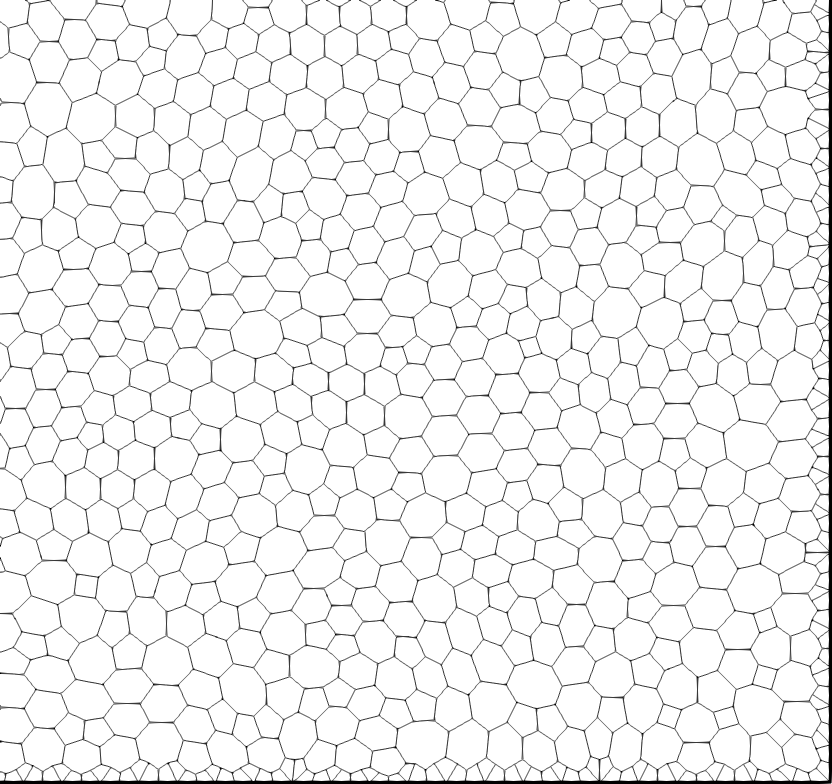
\includegraphics[width=0.30\textwidth]{\myGraphs/statObjImgs/polyMeshV2.png}};
\node [anchor=east,left] (triMeshFig) at (polyMeshFig.west) {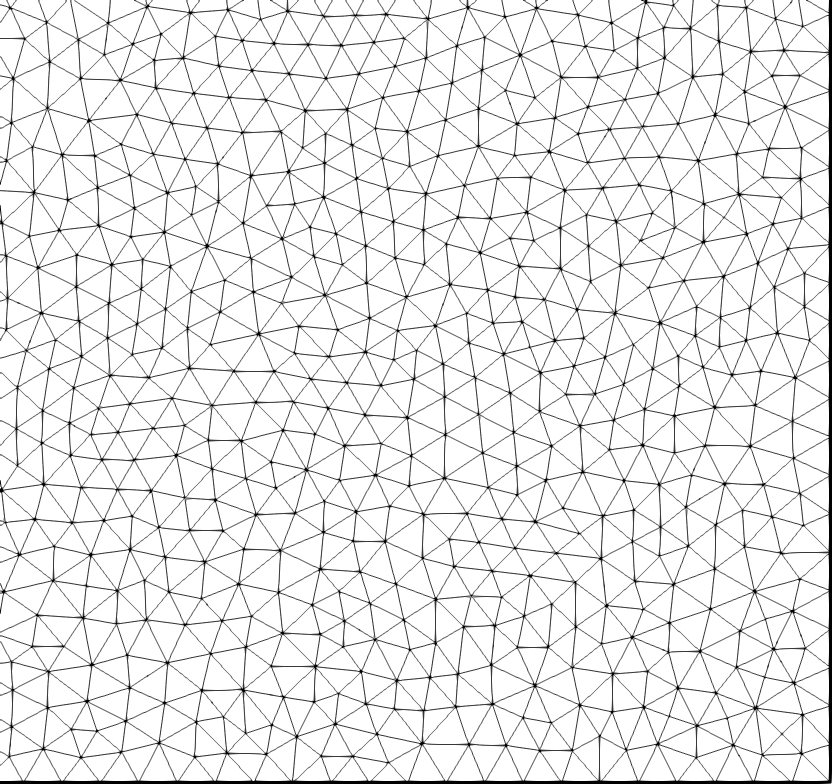
\includegraphics[width=0.30\textwidth]{\myGraphs/statObjImgs/triMeshV2.png}};
\node [anchor=east,left] (hexMeshFig) at (triMeshFig.west) {
\includegraphics[width=0.30\textwidth]{\myGraphs/statObjImgs/hexMeshV2.png}};

%~ \node [right=-1.35cm,anchor=south west] (hexMeshFig) at (statSphere.above north west) {
\includegraphics[width=0.30\textwidth]{\myGraphs/statObjImgs/hexMeshV2.png}};
%~ \node [right=-0.55cm,anchor=south] (triMeshFig) at (statSphere.above north) {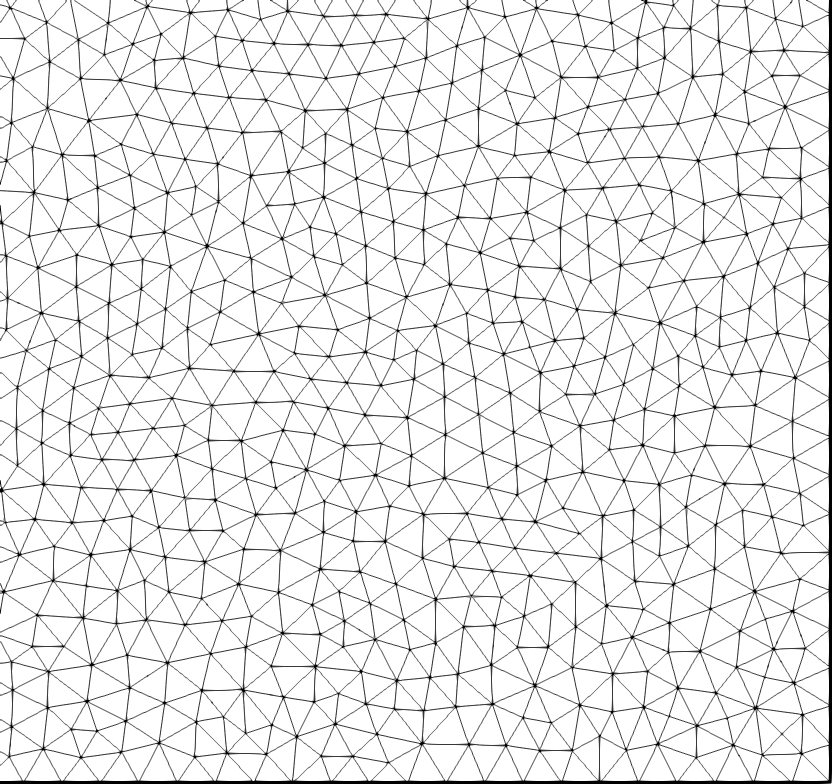
\includegraphics[width=0.30\textwidth]{\myGraphs/statObjImgs/triMeshV2.png}};
%~ \node [right=0.05cm,anchor=south east] (polyMeshFig) at (statSphere.above north east) {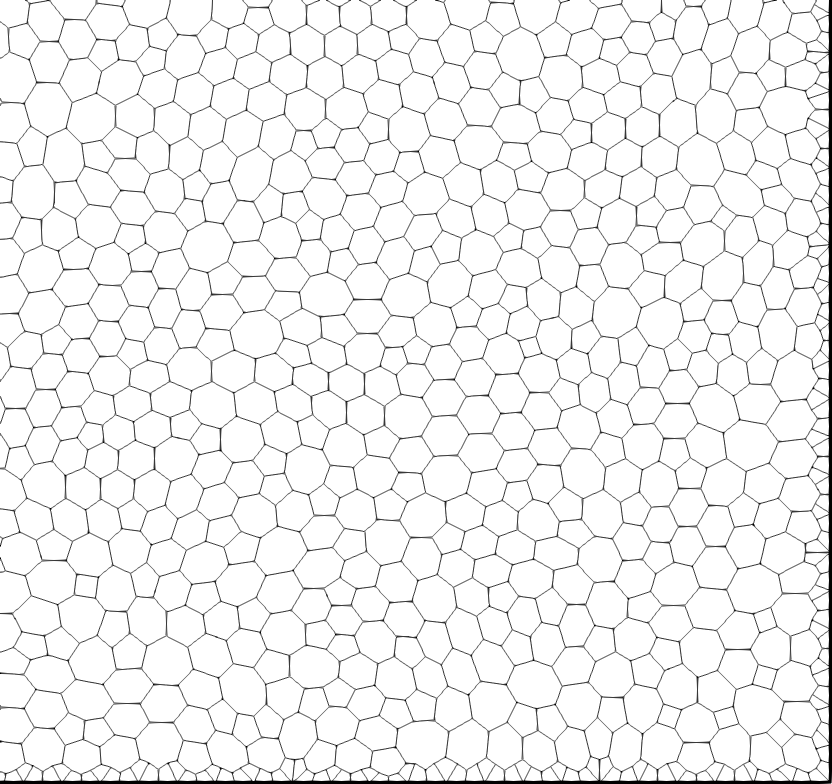
\includegraphics[width=0.30\textwidth]{\myGraphs/statObjImgs/polyMeshV2.png}};

\node [anchor=south, above = -0.1cm of hexMeshFig] (hexMeshText) {hexMesh};
\node [anchor=south, above = -0.1cm of triMeshFig] (triMeshText) {triMesh};
\node [anchor=south, above = -0.1cm of polyMeshFig] (polyMeshText) {polyMesh};

\end{tikzpicture}
